\documentclass[a4paper, 12pt, oneside]{article} % A4 paper size, default 11pt font size and oneside for equal margins

\newcommand{\plogo}{\fbox{$\mathcal{PL}$}} % Generic dummy publisher logo
\usepackage[margin=0.5in]{geometry}
\usepackage[utf8]{inputenc} % Required for inputting international characters
\usepackage{booktabs}
\usepackage{graphicx}
\usepackage[T1]{fontenc} % Output font encoding for international characters
\usepackage{fouriernc} % Use the New Century Schoolbook font
\usepackage{setspace}
\usepackage{enumerate}
%----------------------------------------------------------------------------------------
%	TITLE PAGE
%----------------------------------------------------------------------------------------

\begin{document} 

\begin{titlepage} % Suppresses headers and footers on the title page

	\centering % Centre everything on the title page
	
	\scshape % Use small caps for all text on the title page
	
	\vspace*{2\baselineskip} % White space at the top of the page
	
	%------------------------------------------------
	%	Title
	%------------------------------------------------
	
	\rule{\textwidth}{1.6pt}\vspace*{-\baselineskip}\vspace*{2pt} % Thick horizontal rule
	\rule{\textwidth}{0.4pt} % Thin horizontal rule
	
	\vspace{0.75\baselineskip} % Whitespace above the title
	
	{\LARGE EECS 464 HANDS ON ROBOTICS\vskip 0.2in PROJECT 0 FINAL REPORT} % Title
	
	\vspace{0.75\baselineskip} % Whitespace below the title
	
	\rule{\textwidth}{0.4pt}\vspace*{-\baselineskip}\vspace{3.2pt} % Thin horizontal rule
	\rule{\textwidth}{1.6pt} % Thick horizontal rule
	\vspace{3\baselineskip}
	\begin{figure}[htbp]
		\centering
		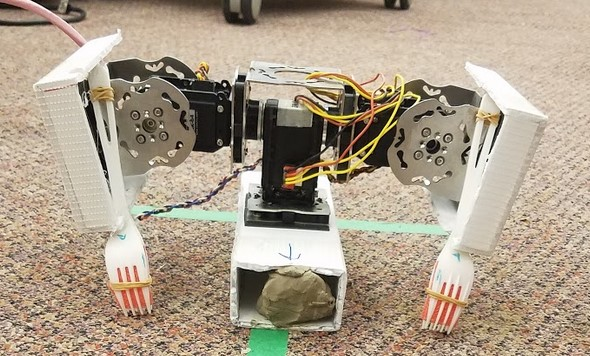
\includegraphics[width=10cm]{cover.jpg}
	\end{figure}
	\vspace{2\baselineskip} % Whitespace after the title block
	
	
	%------------------------------------------------
	%	Editor(s)
	%------------------------------------------------
	
	Edited By Team Blue
	
	\vspace{0.5\baselineskip} % Whitespace before the editors
	
	{\scshape\Large Royce Chung \\ Anne Gu \\ Mukai Wang \\ Ali Yassin} % Editor list
	
	\vfill

	
	\today
	

	

\end{titlepage}
\pagenumbering{gobble}
\begin{spacing}{1.5}
\tableofcontents
\end{spacing}
\newpage
\setcounter{page}{1}
\pagenumbering{Roman}
\section{Background}
\subsection{Problem Description}
The main object of this project is to build a robot that is able to navigate around a figure eight track as fast as possible without being disqualified. The basic requirements include:
\begin{enumerate} 
\item The robot can move 1 meter forward 
\item The robot can rotate 90 degrees 
\item Fits in a 60 x 15 x 30 cm box.
\end{enumerate} 
Some of the constraints that need to be considered are:
\begin{enumerate} 
\item Only three Dynamixel motors are allowed 
\item No fully rotational parts are allowed 
\item The track is carpeted 
\item The robot is tethered by controller.
\end{enumerate} 
\subsection{Brainstorming}

\subsection{Alternative Prototypes}
\subsection{Final Design}
\begin{itemize}
	
	\item \textbf{Mechanical Part}
		\newline
		 
	\item \textbf{Programming Part}\newline
		In the code, we prepare three different motion plans: moving forward, turing left and turning right. Every plan is a cycle with a period of 1 second, and we can hold keys on the keyboard to repeat different motion plans and achieve the leaping and turning function. The three motion plans are shown below. "M" stands for middle servo, "L" stands for the servo on the left(from the rear view), and "R" stands for the servo on the right(from the rear view).
		\begin{table}[htbp]
			\begin{minipage}{0.33\textwidth}
				\centering
				\begin{tabular}{cccc}
					\hline
					t(s) & M($^{\circ}$) & L($^{\circ}$) & R($^{\circ}$)\\
					\hline
					0.05&0&10&10\\
					0.1&-5&10&10\\
					0.15&-10&10&10\\
					0.2&-15&10&10\\
					0.25&-20&10&10\\
					0.3&-25&10&10\\
					0.35&-30&10&10\\
					0.4&-35&10&10\\
					0.45&-40&10&10\\
					0.5&-45&10&10\\
					0.55&-50&10&10\\
					0.6&-55&10&10\\
					0.65&-55&10&10\\
					0.7&-55&10&10\\
					0.75&-55&10&10\\
					0.8&-55&10&10\\
					0.85&-55&10&10\\
					0.9&-55&10&10\\
					0.95&0&10&10\\
					\hline
				\end{tabular}
				\caption{Forward}
			\end{minipage}
			\begin{minipage}{0.33\textwidth}
				\centering
				\begin{tabular}{cccc}
					\hline
					t(s) & M($^{\circ}$) & L($^{\circ}$) & R($^{\circ}$)\\
					\hline
					0.05&0&10&-90\\
					0.1&-5&10&-90\\
					0.15&-10&10&-90\\
					0.2&-15&10&-90\\
					0.25&-20&10&-90\\
					0.3&-25&10&-90\\
					0.35&-30&10&-90\\
					0.4&-35&10&-90\\
					0.45&-40&10&-90\\
					0.5&-45&10&-90\\
					0.55&-50&10&-90\\
					0.6&-55&10&-90\\
					0.65&-55&10&-90\\
					0.7&-55&10&-90\\
					0.75&-55&10&-90\\
					0.8&-55&10&-90\\
					0.85&-55&10&-90\\
					0.9&-55&10&-90\\
					0.95&0&10&-90\\
					\hline
				\end{tabular}
				\caption{Turn Left}
			\end{minipage}
			\begin{minipage}{0.33\textwidth}
				\centering
				\begin{tabular}{cccc}
					\hline
					t(s) & M($^{\circ}$) & L($^{\circ}$) & R($^{\circ}$)\\
					\hline
					0.05&0&-90&10\\
					0.1&-5&-90&10\\
					0.15&-10&-90&10\\
					0.2&-15&-90&10\\
					0.25&-20&-90&10\\
					0.3&-25&-90&10\\
					0.35&-30&-90&10\\
					0.4&-35&-90&10\\
					0.45&-40&-90&10\\
					0.5&-45&-90&10\\
					0.55&-50&-90&10\\
					0.6&-55&-90&10\\
					0.65&-55&-90&10\\
					0.7&-55&-90&10\\
					0.75&-55&-90&10\\
					0.8&-55&-90&10\\
					0.85&-55&-90&10\\
					0.9&-55&-90&10\\
					0.95&0&-90&10\\
					\hline
				\end{tabular}
				\caption{Turn Right}
			\end{minipage}
		\end{table}
	
		When moving forward, the middle servo swings the two legs back by 55 degrees. This motion is completed in 1 second. Meanwhile the other two servos fold in by 10 degrees. We realize that leg angles matter after we tested the number of steps needed to leap forward by 1 m by changing the angles. In the test, the angles that we picked are 0, 10 and 20 degrees. The result is in table \ref{ttest}.
		\begin{table}[htbp]
			\centering
			\begin{tabular}{ccc}
				\toprule
				$0^{\circ}$&$10^{\circ}$&$20^{\circ}$\\
				\midrule
				11&	9&	9\\
				11&	9&	11\\
				11&	9&	10\\
				11&	10&	9.5\\
				11&	9.5&10\\
				\bottomrule
			\end{tabular}
		\caption{Number of Steps to Leap Forward by 1m}\label{ttest}
		\end{table}
	  
		We apply t-test with 4 degrees of freedom to comparing the case of $0^{\circ}$ and $10^{\circ}$ and comparing the case of $10^{\circ}$ and $20^{\circ}$. When comparing $0^{\circ}$ and $10^{\circ}$, we had a p-value of 0.001, which is much smaller than 0.05. This is sufficient to reject the null hypothesis of equality and conclude that the legs leap faster when it is folded in by $10^{\circ}$ than $0^{\circ}$. When comparing $10^{\circ}$ and $20^{\circ}$, we had a p-value of 0.235. This is not sufficient to reject the null hypothesis, so we should say the folding legs by $10^{\circ}$ has the same performance as $20^{\circ}$ in terms of speed. We pick $10^{\circ}$ to ensure that more teeth of the fork legs are touching the ground. It can mitigate the chances that the teeth break when the robot is leaping forward.
		
		As to moving left, the left servo and the middle servo follow the same pattern as they are when the robot is moving forward. The right servo swings to -90 degrees to raise the right foot in the air. We do this to make sure it doesn't interfere when the left leg is dragging the body rightwards.
		
		Turning right follows the same philosophy as turning left. The only difference lies in that the motions of the left and right servos are swapped. 
\end{itemize}
\section{Result}
P-day has four different events. First was the qualification round where the robot had to move from one end of the track to the other in a line ignoring the marker tape. The next event was a race around the figure eight track with inner and outer bounds. The third event was the same as the previous, but only the inner bound applied. The last event was a straight race along a 15’ straightaway.
\subsection{Qualification}
\subsection{Figure Eight Track (Inner and Outer Bounds)}
\begin{table}[htbp]
	\centering
	\begin{tabular}{c|ccccc}
		&Trial 1&Trial 2&Trial3&Trial4&Trial5\\
		\hline
		Green Team &134 (DQ)& 143& &111(DQ)& 133\\
		
		Red Team& & 76 (DQ)&67& &63\\
		
		
		Blue Team& 160 (DQ)& &153 (DQ)& 127& \\
		
	\end{tabular}
\end{table}
\subsection{Figure Eight Track (Only Inner Bounds)}
\begin{table}[htbp]
	\centering
	\begin{tabular}{c|ccccc}
		&Trial 1& Trial 2& Trial 3& Trial 4& Trial 5\\
		\hline 
		Green Team&& 140 (DQ)&110 (DQ)&&83\\
		Red Team& 63&& 65& 61& 44\\
		Blue Team& 151& 153 (DQ)& &166 (DQ)&\\
	\end{tabular}
\end{table}
\subsection{15’ Straightaway Race}
\begin{table}[htbp]
	\centering
	\begin{tabular}{c|ccccc}
		&Trial 1 &Trial 2 &Trial 3 &Trial 4& Trial 5\\
		\hline 
		Green Team&&DNF&&38&38\\
		Red Team&39&69&44&&42\\
		Blue Team& 76&&73&54&\\
	\end{tabular}
\end{table}
\section{Discussion}

\subsection{Project Day Result Analysis}
\begin{itemize}
	\item Turning was time consuming. Takes approximately 7 seconds to turn 90 degrees either right or left. Turns were primarily the reason why we got disqualified so often. Improvements can include adding features to the side of the fork, such as bamboo skewers or knives. 
	\item Our robot slipped a lot. Localized, Friction based movements. Especially on tape. The back end of the base of our robot, ended up adding a knife at the end to help prevent the slipping. Using the leg padding from the other team, helped us realize that directional friction was needed, but ultimately using the padding prevented us from turning.
	\item Our robot’s stride length and stride times were slow compared to other teams. 
\end{itemize}
\subsection{Future work}
\end{document}